\documentclass[10pt,a4paper]{amsart}
\usepackage[margin=19mm]{geometry}
\usepackage{amsmath,amssymb,mathtools}
\usepackage[scr=rsfs,cal=euler]{mathalfa}
\usepackage{xfrac}
\usepackage[unicode,hidelinks,bookmarks=false]{hyperref}
\newcommand{\ie}{i.e.\ }
\newcommand{\cf}{cf.\ }
\newcommand{\resp}{respectively\ }
\newcommand{\Subsection}{\subsection}
\providecommand{\nobreakdash}{\nobreak\hbox{-}}
\setlength{\emergencystretch}{2em}
\multlinegap0pt
\usepackage{tikz}
\usepackage{float}
\usepackage{amssymb}
\usepackage{braket}
\usepackage{dsfont}
\usepackage{enumerate}
\usepackage{mathtools}
\newtheorem{lemma}{Lemma}
\newcommand{\Nc}{\mathcal{N}}
\newcommand{\R}{\mathbb{R}}
\newcommand{\Sb}{\mathbb{S}}
\DeclareMathOperator{\dist}{dist}
\title{Spherical harmonics and point configurations on the sphere}
\author{Xiaolong Han}
\date{Source: arXiv:2209.03403v3 (CC BY 4.0)}
\begin{document}
\maketitle

\noindent\emph{Source and licence.} Spherical harmonics and point configurations on the sphere. Version arXiv:2209.03403v3 (CC BY 4.0), distributed by arXiv under the Creative Commons Attribution 4.0 International licence, http://creativecommons.org/licenses/by/4.0/, as recorded in the arXiv licence metadata for this exact version and shown on the abstract page https://arxiv.org/abs/2209.03403v3. Full licence notice: \texttt{licenses/arxiv-2209.03403-CC-BY-4.0.txt}.\par\smallskip

\noindent\textit{Editorial scope.} Counted unit: the article's lemma lemma:cover (source0.tex lines 770--772). The article's complete original proof of it is delivered with it (source0.tex lines 774--802, one \texttt{proof} environment of 29 lines). No mathematics is written, repaired or re-derived: the statement and the proof are the article's own lines, in the article's own notation, and no retained line is substituted or re-flowed.  Retained uncounted as the source-local context the proof needs: lines 807--828.  Nothing was omitted from any retained span, so the package carries no omission record.  No retained line contains a citation, so the wrapper carries no bibliography and no bibliography entry.  The retained lines contain the article's own diagram code, which the wrapper typesets with the standard tikz packages; no image file is delivered and the package declares no asset dependency.  Editorial formatting only, in addition: an AMS \texttt{amsart} preamble that restates the article's own declarations and macros used by the retained lines, namely the environments \texttt{lemma} on separate counters, together with the standard packages those lines need.  The retained environments print in this document as Lemma 1 in order of appearance, whereas the article prints the same items with the numbering of its own full document.  The complete native source of the article as distributed in the arXiv e-print for this exact version is bundled unchanged as \texttt{sources/130421/source0.tex}.
\begin{figure}[H]
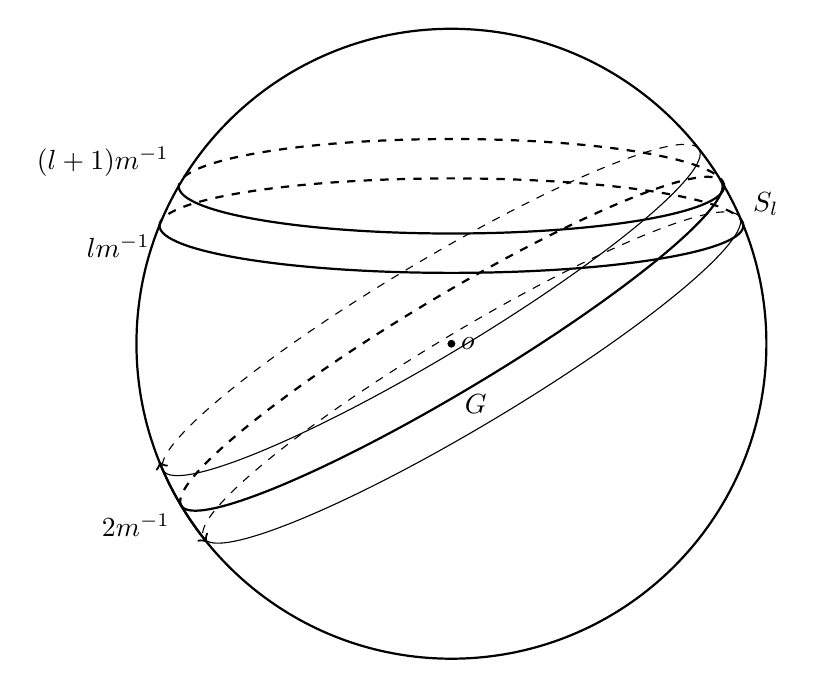
\begin{tikzpicture}
\draw[thick] (0,0) circle (4);
\fill[] (0,0) circle (0.05cm) node[right]{$o$};
\draw[thick] (-3.708,1.5) arc (180:360:3.708 and 0.6);
\draw[thick,dashed] (3.708,1.5) arc (0:180:3.708 and 0.6);
\draw[thick] (-3.464,2) arc (180:360:3.464 and 0.6);
\draw[thick,dashed] (3.464,2) arc (0:180:3.464 and 0.6);
\draw[rotate around={0.54r:(0,0)},thick] (-4,0) arc (180:360:4 and 0.6) node[below,midway]{$G$};
\draw[rotate around={0.54r:(0,0)},thick,dashed] (-4,0) arc (180:0:4 and 0.6);
\draw[rotate around={0.54r:(0,0)}] (-3.967,0.5) arc (180:360:3.967 and 0.6);
\draw[rotate around={0.54r:(0,0)},dashed] (3.967,0.5) arc (0:180:3.967 and 0.6);
\draw[rotate around={0.54r:(0,0)}] (-3.967,-0.5) arc (180:360:3.967 and 0.6);
\draw[rotate around={0.54r:(0,0)},dashed] (3.967,-0.5) arc (0:180:3.967 and 0.6);
\draw[thick,<->] (-3.708,-1.5) arc (202:219:4) node[anchor=north east,midway]{$2m^{-1}$};
\draw (3.708,1.5) node[anchor=south west]{$S_l$};
\draw[] (-3.708,1.5) node[anchor=north east]{$lm^{-1}$};
\draw[] (-3.464,2) node[anchor=south east]{$(l+1)m^{-1}$};
\end{tikzpicture}
\caption{Intersection of a latitudinal strip $S_l$ and $\Nc_{m^{-1}}(G)$, where $G$ forms an angle of $(l+1)m^{-1}$ with the equator $G_0$.}
\label{fig:strip}
\end{figure}

\begin{lemma}[Covering of latitudinal strips]\label{lemma:cover}
Let $m\ge6$ and $1\le l\le\frac m3$. Then $S_l$ is contained in the union of the $m^{-1}$-neighborhoods $\Nc_{m^{-1}}(G)$ of at most $5(l+1)$ great circles $G\subset\Sb$.
\end{lemma}

\begin{proof}
We identify the points of $\Sb$ with unit vectors in $\R^3$, so that $\langle x,y\rangle=\cos\dist(x,y)$ for $x,y\in\Sb$. Since the great circle $G_p$ with pole $p$ consists of the points at distance $\frac\pi2$ from $p$,
$$\dist\left(x,G_p\right)=\left|\frac\pi2-\dist(x,p)\right|=\left|\arcsin\left\langle x,p\right\rangle\right|\quad\text{for }x\in\Sb.$$
Because $m^{-1}\le\frac\pi2$, it follows that
\begin{equation}\label{eq:nbhd}
x\in\Nc_{m^{-1}}\left(G_p\right)\quad\text{if and only if}\quad\left|\left\langle x,p\right\rangle\right|\le\sin\frac1m.
\end{equation}
Let $G$ be the great circle forming the angle $(l+1)m^{-1}$ with the equator $G_0$ whose highest point has longitude $0$; see Figure \ref{fig:strip}. Its pole is then
$$p=\left(-\sin\frac{l+1}{m},0,\cos\frac{l+1}{m}\right),$$
and
$$\frac{l+1}{m}\le\frac13+\frac16=\frac12,$$
since $l\le\frac m3$ and $m\ge6$.

Let $x\in S_l$ have latitude $\alpha$ and longitude $\theta$ with $|\theta|\le(l+1)^{-1}$. In our coordinates,
\begin{eqnarray*}
\left\langle x,p\right\rangle&=&-\cos\alpha\cos\theta\sin\left(\frac{l+1}{m}\right)+\sin\alpha\cos\left(\frac{l+1}{m}\right)\\
&=&-\sin\left(\frac{l+1}{m}-\alpha\right)+\cos\alpha\sin\left(\frac{l+1}{m}\right)\left(1-\cos\theta\right).
\end{eqnarray*}
Since $lm^{-1}\le\alpha<(l+1)m^{-1}$ for $x\in S_l$, the first term satisfies
$$0<\sin\left(\frac{l+1}{m}-\alpha\right)\le\sin\frac1m.$$
Moreover, by $\sin\beta\le\beta$ and $1-\cos\beta\le\frac{\beta^2}{2}$,
$$0\le\cos\alpha\sin\frac{l+1}{m}\left(1-\cos\theta\right)\le\frac{l+1}{m}\cdot\frac{1}{2(l+1)^2}\le\frac{1}{2m}\le\sin\frac1m,$$
where in the last inequality we used $\sin\beta\ge\frac{2\beta}{\pi}\ge\frac\beta2$ for $0\le\beta\le\frac\pi2$. Combining the last three displays,
$$\left|\left\langle x,p\right\rangle\right|\le\sin\frac1m,$$
and therefore $x\in\Nc_{m^{-1}}(G)$ by \eqref{eq:nbhd}.

Thus $\Nc_{m^{-1}}(G)$ contains all points of $S_l$ whose longitude lies within $(l+1)^{-1}$ of $0$. Set $K=\lceil\pi(l+1)\rceil$ and rotate $G$ about the polar axis by the angles $\frac{2\pi k}{K}$, $k=1,...,K$. Every longitude lies within $\frac\pi K\le\frac{1}{l+1}$ of $\frac{2\pi k}{K}$ modulo $2\pi$ for some $k$, while $S_l$ is invariant under rotations about the polar axis. Hence these great circles cover $S_l$, and their number is
$$K\le\pi(l+1)+1\le5(l+1).$$
\end{proof}

\end{document}
